\chapter{Ajout d'une singularité dans le réseau}
La seconde partie de ce projet est une étude portant sur l'observation d'un mode localisé dans le réseau précédemment étudié. Pour cela, un résonateur est modifié de façon à créer une singularité dans le réseau. \\
Le banc de manipulation ne nous permet de modifier que la longueur des cavités des résonateurs et non leur position. C'est donc en changeant ce paramètre que sera introduite et étudiée la singularité. La longueur de la cavité singulière est notée $L_{c_{s}}$.\\

En fonction du choix de la longueur de la cavité singulière, et donc de la fréquence de résonance du résonateur associé, différents phénomènes peuvent être observés. 

\section{Étude de l'influence de la fréquence de résonance du défaut}
Le réseau étudié à un comportement complexe d'un point de vue fréquentiel. Il est donc important de différentier différents cas suivant la fréquence de résonance du défaut. Les 2 cas de figures sont représentés sur le schéma \ref{schema_singu1}.

\begin{figure}[!h]
\centering
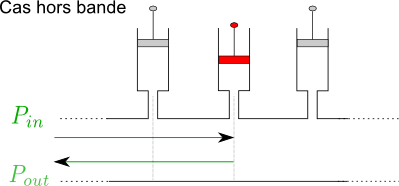
\includegraphics[scale=0.5]{images_chp2/schema_singu1.png} \hfill
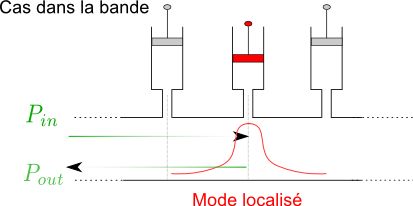
\includegraphics[scale=0.5]{images_chp2/schema_singu2.png}
\caption{\label{schema_singu1} Schémas de la configuration avec une singularité dans une bande interdite  et hors bande interdite.}
\end{figure}



 




\subsection{Cas du défaut hors bandes interdites}
Le cas le plus simple d'une singularité dans le réseau est celui ou cette singularité se trouve hors de la bande de Bragg ou des bandes liés aux autres résonateurs (la fréquence de résonance du réseau ne se trouve pas dans la bande). La singularité agit comme un mur dans le réseau à sa fréquence de résonance car alors l'impédance du résonateur est maximale. Dans ce cas, la pression dans le réseau après la singularité est nulle. Ce résultat se retrouve lors des simulations. On trace sur la figure ~\ref{defaut_hb} la simulation de la pression dans le réseau ainsi que le coefficient de transmission.


\begin{figure}[!h]
\centering
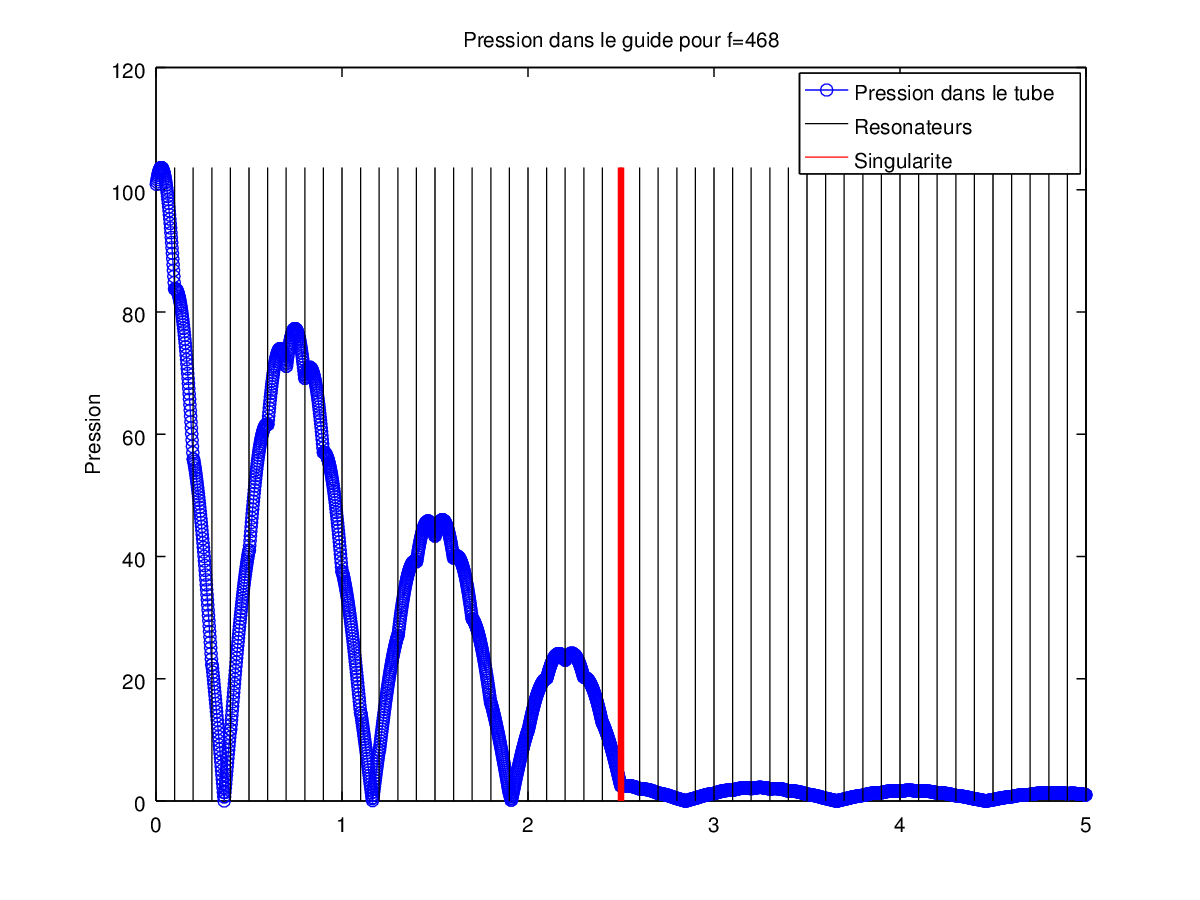
\includegraphics[scale=0.5]{images_chp2/visu_pression_defavo.png}
\caption{\label{defaut_hb} Visualisation de la pression dans le réseau avec un défaut dont la fréquence se trouve hors d'une bande interdite. La fréquence d'excitation est celle du défaut. Celui-ci se trouve en 25eme position dans un réseau de 50 résonateurs.}
\end{figure}

\bigskip
On constate bien une coupure de la pression au niveau de la singularité. Le défaut à théoriquement une impédance infinie à la résonance, il y a donc une réflexion totale. Ici, les pertes sont prisent en comptes, une fraction de l'onde incidente se propage donc dans le réseau car l'impédance n'est pas infinie, d'où la légère oscillation visible.



\subsection{Cas du défaut dans une bande interdite}

Dans les autres cas (résonance du défaut dans une bande interdites) des phénomènes plus complexes apparaissent.
Si la fréquence de résonance du défaut se trouve dans une bande interdite, on a alors une localisation de l'onde au niveau du défaut. En effet la propagation n'est pas possible dans le réseau, on a donc des ondes évanescentes, la fraction de l'onde incidente qui c'est propagé jusqu'au défaut excite sa résonance mais reste piégé du fait que ce défaut se trouve au milieu du réseau. On obtient alors un mode localisé: la pression est élevée à un endroit du tube et reste confinée.
\bigskip


Du fait que cette pression soit localisée, elle n'a pas d'influence sur les coefficients de réflexions et transmissions sauf dans le cas d'un petit réseau ou on peut supposer que l'étalement du mode localisé est suffisamment grand au regarde de la taille du réseau pour atteindre les bords de celui-ci. Ce genre de phénomène est donc difficile à observer; cependant une simulation peut aider à en comprendre les concepts clés.
\bigskip

On trace sur la figure \ref{defaut_b} la pression dans le tube pour un défaut dans une bande interdite. Dans cette simulation on reconstruit la pression en chaque points du réseau par rétro-propagation en partant d'une terminaison anéchoïque à la fin du réseau. Les valeurs qu'on peut voir au début du réseau n'ont donc pas nécessairement de réalité physique, on s'intéresse ici surtout à l'enveloppe du signal plus qu'aux ordres de grandeurs.


\todo{tracer le truc}

Il est a noter que la fréquence de résonance du défaut ne correspond pas nécessairement à la fréquence du mode localisé. En effet, celui-ci résulte du défaut couplé avec le reste du réseau, les fréquences de résonances peuvent donc changer.


\section{Étude de l'influence de la position du défaut}
On s’intéresse maintenant à l'influence de la position du défaut dans le réseau.




Toute la troisième partie de ce projet va consister à visualiser expérimentalement un mode localisé.
